%%%%%%%% this is our results and comparison

%\documentclass[12pt, amstex, letterpaper] {report} %{article}


\usepackage[margin=1in]{geometry}
\topmargin -0.5in \textwidth 6.5in \textheight 9in
\footskip .5in
\headheight 0.3in


\usepackage{Sweave}

\DefineVerbatimEnvironment{Sinput}{Verbatim} {xleftmargin=0em,frame=single}
\DefineVerbatimEnvironment{Soutput}{Verbatim} {xleftmargin=0em,frame=single}

\usepackage{amssymb, mathrsfs, amsmath, amsfonts}
\usepackage{enumerate, comment}
\usepackage{hyperref, natbib,apalike, float} %cite
\usepackage{color, multirow, setspace, fancyhdr,graphicx}
\usepackage{undertilde}
\usepackage[bottom]{footmisc}
\usepackage{graphicx}
\usepackage{framed}
\usepackage{subcaption}
\usepackage{amsthm}

%\doublespacing
\pagestyle{empty}
\pagestyle{fancy}
\lhead{ }
%\rhead{May 2016}
\fancyfoot{ }
\rfoot{Dissertation $|$ \thepage}
\lfoot{Chris Vanlangenberg}
\date{}

\includecomment{comment}

\newtheorem{theorem}{Theorem}[section]
\newtheorem{defn}{Definition}[section]
\newtheorem{prop}{Proposition}
\newcommand{\pro}[1]{\begin{prop}{#1}\end{prop}}

%\newtheorem{proof}{proof}
\newtheorem{rmk}{Remark}
\newcommand{\rmark}[1]{\begin{rmk}{#1}\end{rmk}}

\numberwithin{equation}{section}
\renewcommand{\footrulewidth}{0.1pt}
\renewcommand{\headrulewidth}{0.1pt}


\newcommand{\eqn}[1]{\begin{equation}{#1}\end{equation}}

\newcommand{\beq}{\begin{equation}}
\newcommand{\eeq}{\end{equation}}
%\renewcommand\refname{Literature}
\newcommand{\blue}[1]{\textcolor{blue}{\emph{#1}}}
\newcommand{\red}[1]{\textcolor{red}{\emph{#1}}}
\newcommand{\twoc}[2]{{\textcolor{blue}{#1}} and {\textcolor{red}{#2}}}


\newcommand{\xn}{x_1,\ldots, x_n}
\newcommand{\Xn}{X_1,\ldots, X_n}
\newcommand\floor[1]{\lfloor{#1}\rfloor}
\newcommand\ceil[1]{\lceil{#1}\rceil}

\newcommand{\X}{\mathcal{X}}
\newcommand{\Sp}{\mathbb{S}}
\newcommand{\R}{\mathbb{R}}
\newcommand{\C}{\mathbb{C}}
\newcommand{\pd}{positive definite }



\newcommand{\code}[1]{{\small\texttt{#1}}}
\newcommand{\pkg}[1]{{\normalfont\textsf{#1}}}
\newcommand{\var}[1] {{\normalfont\textbf{#1}}}
\newcommand{\Cm}{$C_m(\phi_P, \phi_Q)\ $}

\newcommand{\jun}{\cite{JunStein2008}}
%\begin{document}

To validate if the generated axially symmetric global data follow the given covariance model, we compare the MOM cross variogram estimates from the generated data to its theoretical counterparts. As indicated in Chapter 4, although the cross variogram (\ref{cross_variogram}) only reflects the even component of the cross covariance, it is unbiased. Moreover, when the data are generated from the longitudinally reversible covariance function, the cross variogram is equivalent to the cross covariance. \\

We have conducted the simulation for different pairs of latitudes with the same number of longitudes ($n_L = 100$). The pair of latitudes has been selected from very close by to far away. The cross variogram estimates are almost identical to the theoretical values when the pair of latitudes are closer, which is not shown in the dissertation. Here we demonstrate a case with larger latitude difference ($\phi_P = 10^0, \phi_Q = 150^0$ equivalent to $70^0S$ and $60^0N$) in order to capture the largest possible errors. 

%The rate of convergence (\blue{should we talk about any theoretical properties of convergence since we don't have a proof for consistency}) is very slow as one can see that when number of simulations were increased from 500 to 4000 the cross variogram estimator is much closer to its theoretical value. However, the cross variogram estimator for model 2 and 3 converges much faster compared to model 1.

\vskip 8pt

%-------------------------------------%
\subsection{Comparison of MOM Estimators}
%-------------------------------------%

Now we compare the cross variogram estimates given in $\eqref{cross_variogram}$, using our approach (with $C_m$) and the approach with $R(P,Q)$ directly to generate data, respectively. One can see that the estimate given by our method is closer to the true values than those from $R(P, Q)$ directly, under 500 repetitions and 4000 repetitions respectively (Figure \ref{compare_varigram_sim_1}).

\begin{figure}[H]
	\begin{subfigure}{.5\textwidth}
		\centering
		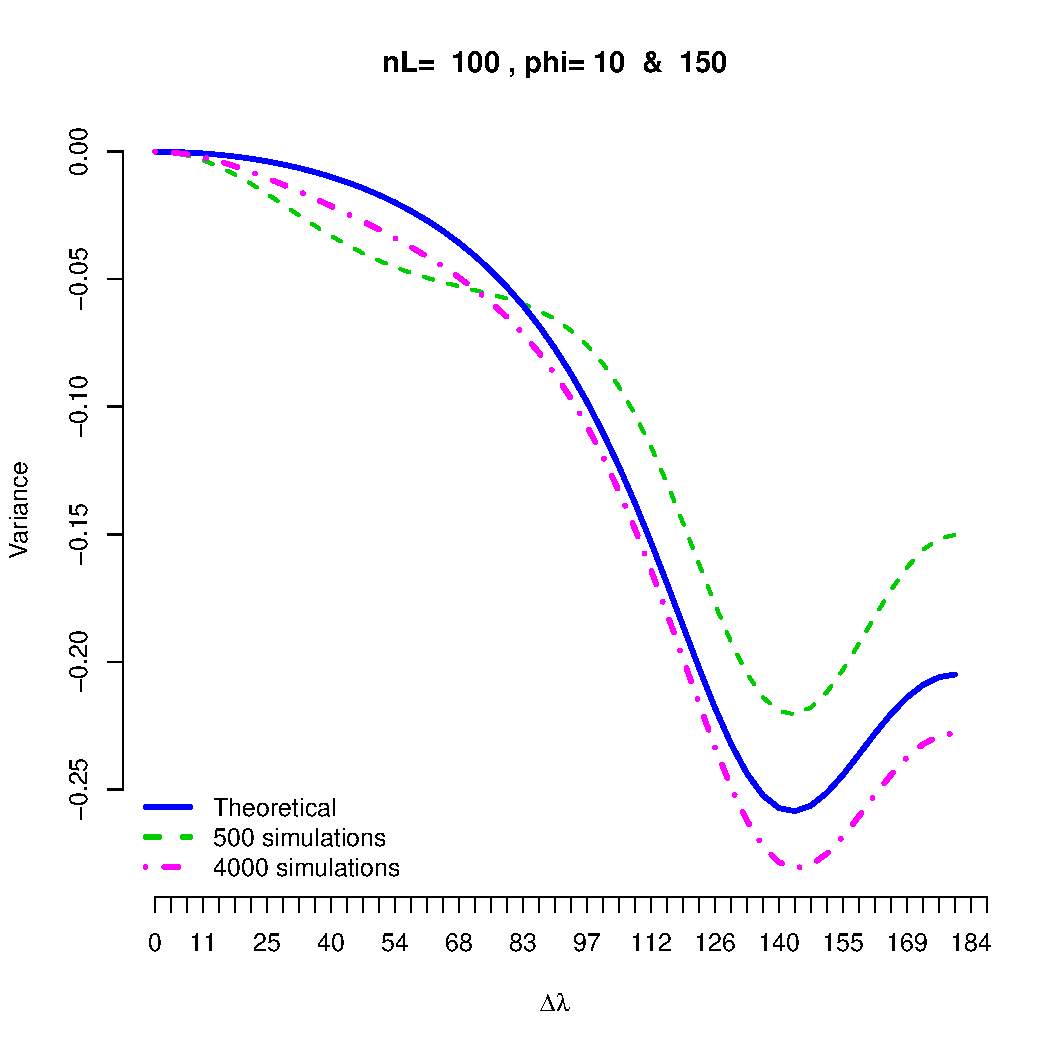
\includegraphics[width=1\linewidth]{graphs/results_variogram_model1_rpq}
		\caption{Using paramter Set 1 and $R(P,Q)$}
		\label{fig:sfig1}
	\end{subfigure}
	\begin{subfigure}{.5\textwidth}
		\centering
		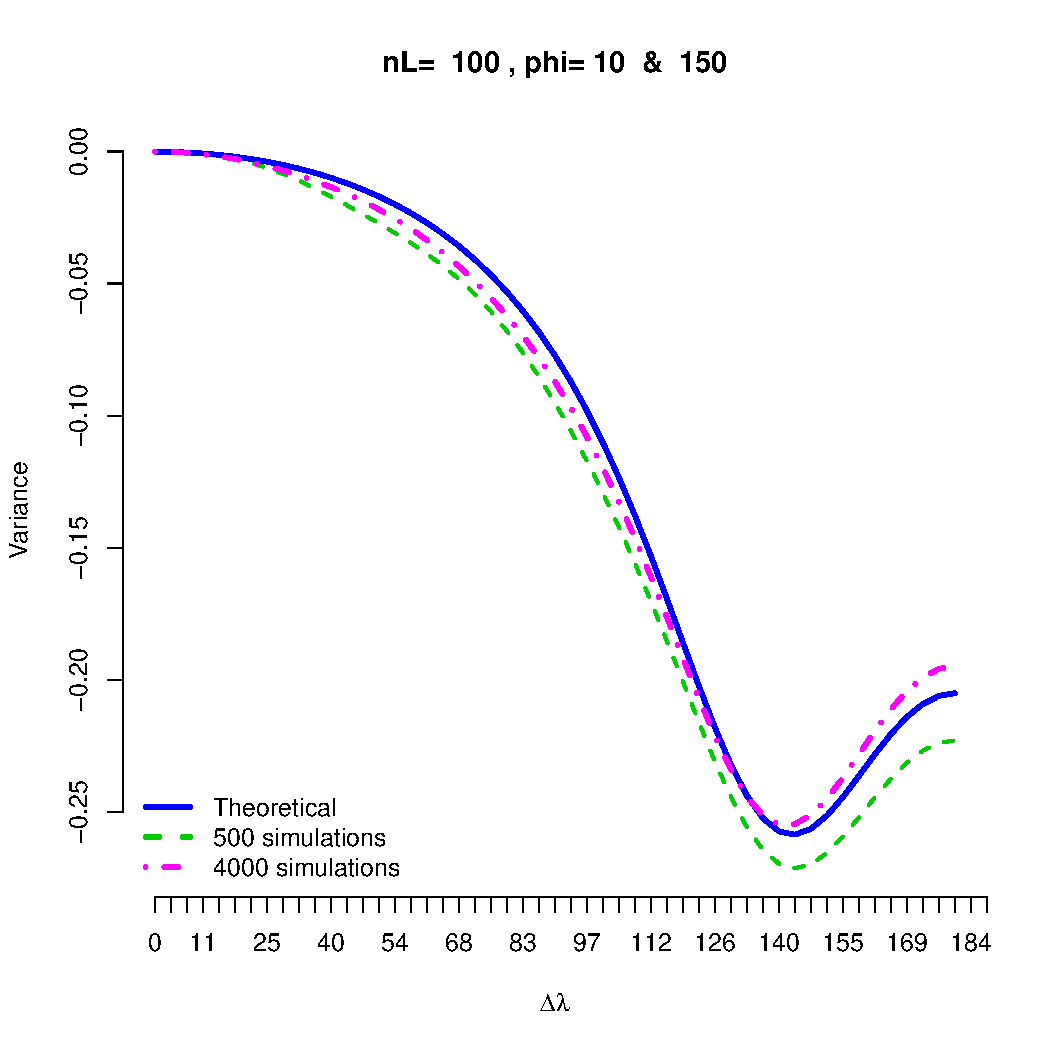
\includegraphics[width=1\linewidth]{graphs/results_variogram_model1}
		\caption{Using paramter Set 1 and $C_m$}
		\label{fig:sfig2}
	\end{subfigure}
	\begin{subfigure}{.5\textwidth}
		\centering
		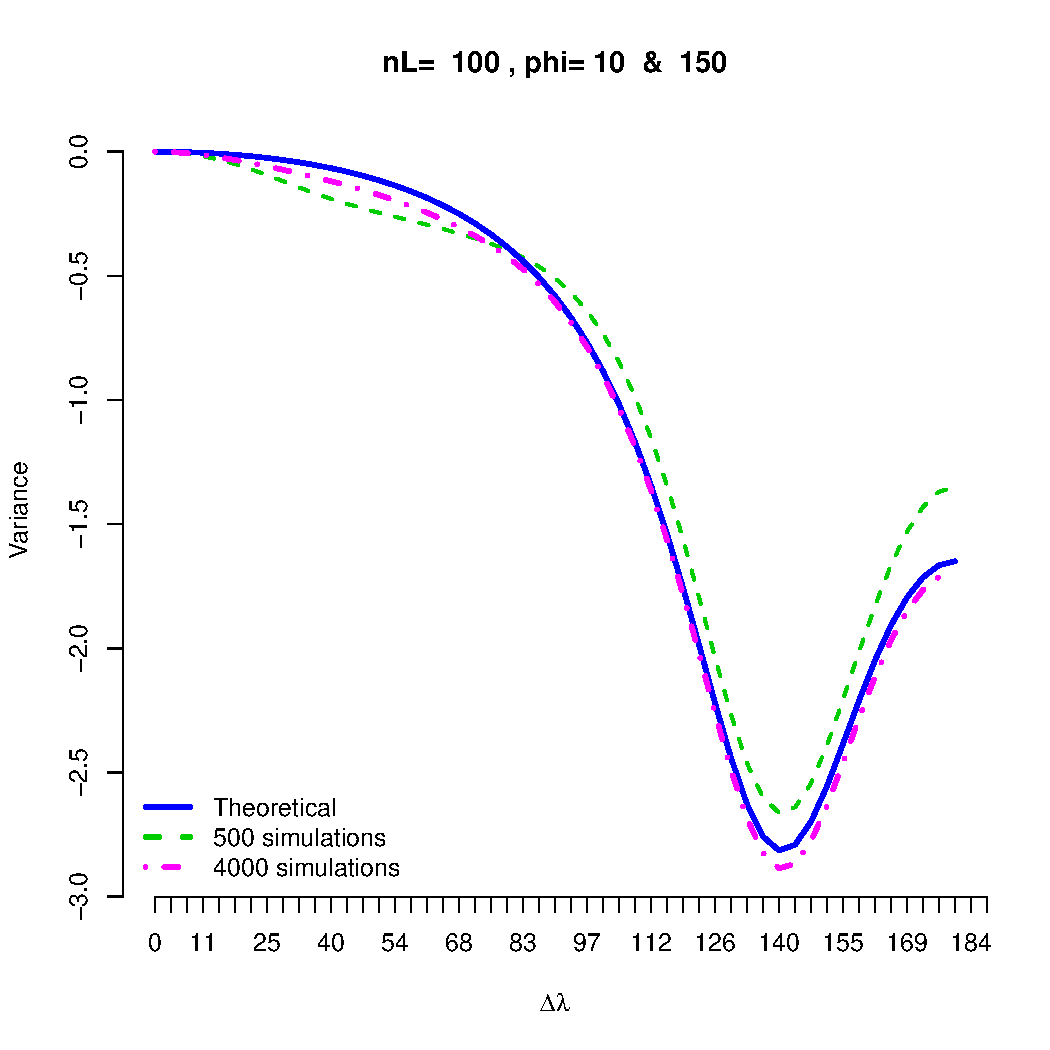
\includegraphics[width=1\linewidth]{graphs/results_variogram_model1_rpq_2}
		\caption{Using paramter Set 2 and $R(P,Q)$}
		\label{fig:sfig1}
	\end{subfigure}
	\begin{subfigure}{.5\textwidth}
		\centering
		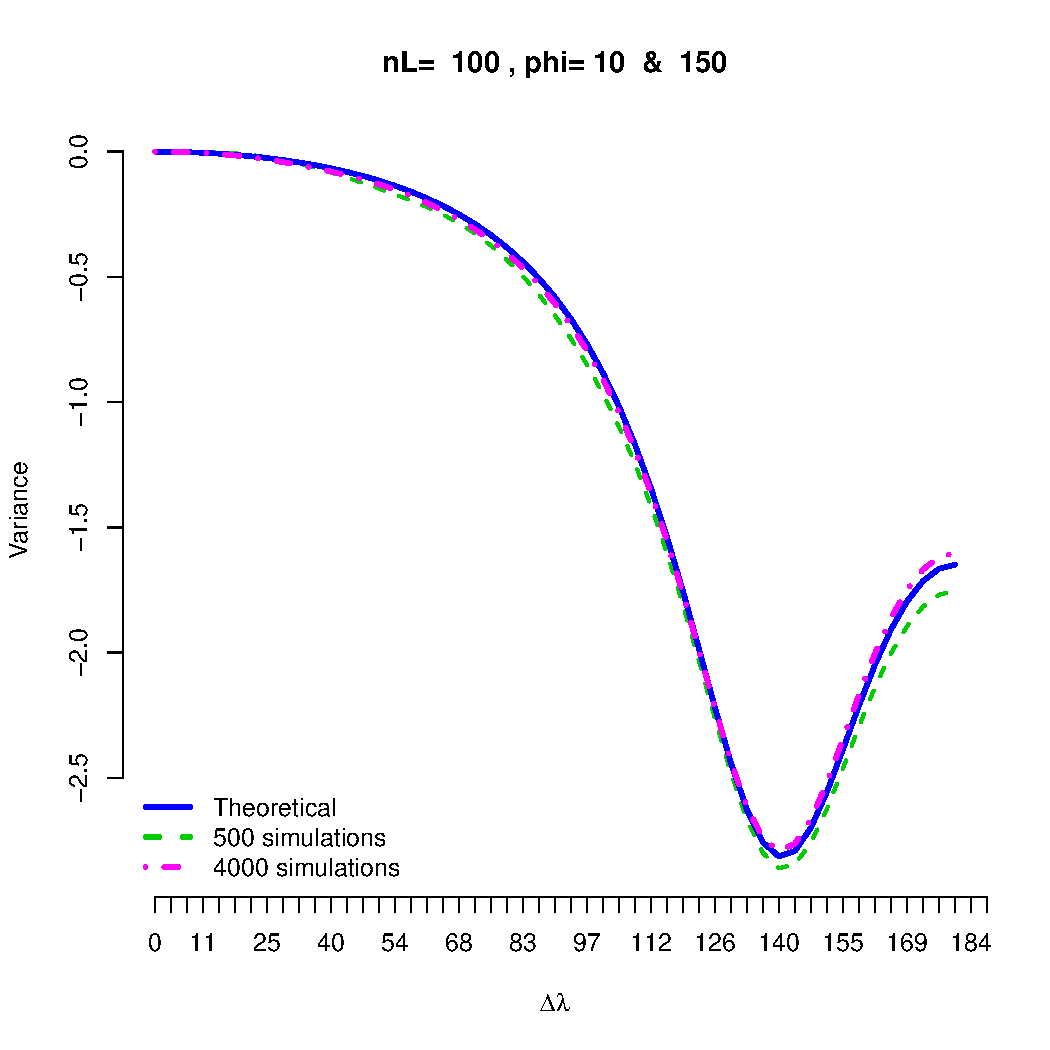
\includegraphics[width=1\linewidth]{graphs/results_variogram_model1_2}
		\caption{Using paramter Set 2 and $C_m$}
		\label{fig:sfig2}
	\end{subfigure}
	\caption[Using Parameter Set 1 and Set 2 to Perform The Variogram Estimator]{Using parameter Set 1 and Set 2 to perform the variogram estimator under model 1, solid line (blue) represents the theoretical values of cross variogram and dashed lines (green, purple) represents the estimates for 500 and 4000 simulations respectively. }
	\label{compare_varigram_sim_1}
\end{figure}


%-------------------------------------%
\subsection{Results for Longitudinally Reversible Processes}
%-------------------------------------%

Setting parameter $u = 0$ in all of our models yields longitudinally reversible covariance functions (see Figure \ref{fig_parameter_comp} 1(d) ). Based on 500 simulations, one can see that the cross variogram estimates from direct $R(P,Q)$ approach are slightly away from the theoretical values all three models (Figure \ref{logitudinal_comparison_rpq}). In contrast from the $C_m$ approach the estimates are very close to theoretical values (Figure \ref{logitudinal_comparison_cm}).

\begin{figure}[H]
	\centering
	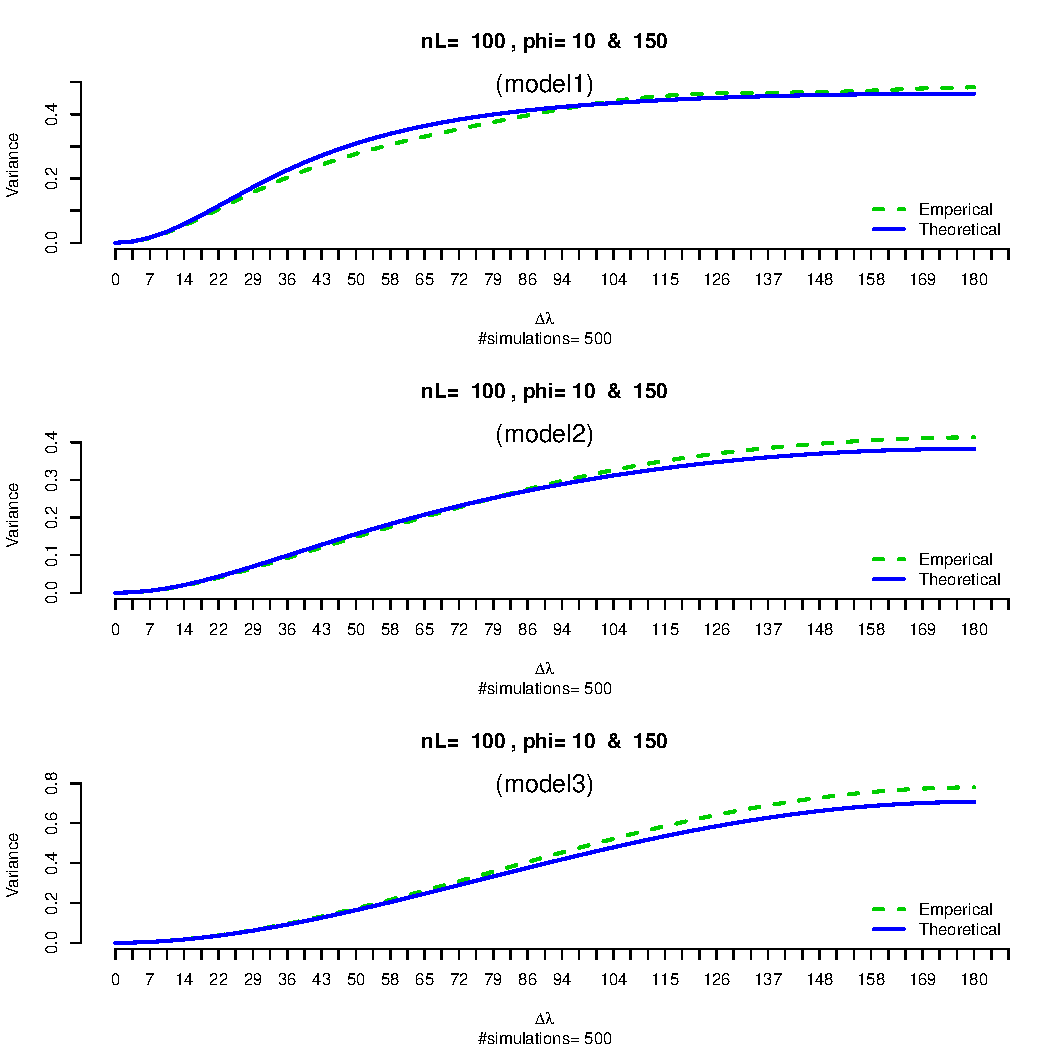
\includegraphics [scale =.9, keepaspectratio]{graphs/results_variogram_comparison_rpq}
	\caption[Based on $R(P,Q)$ Approach the Cross Variogram Estimator Comparison]{Based on $R(P,Q)$ approach the cross variogram estimator comparison for longitudinally reversible process using  model 1, model 2, and model 3 (when $u=0$).}
	\label{logitudinal_comparison_rpq}
\end{figure}

\begin{figure}[H]
	\centering
	% 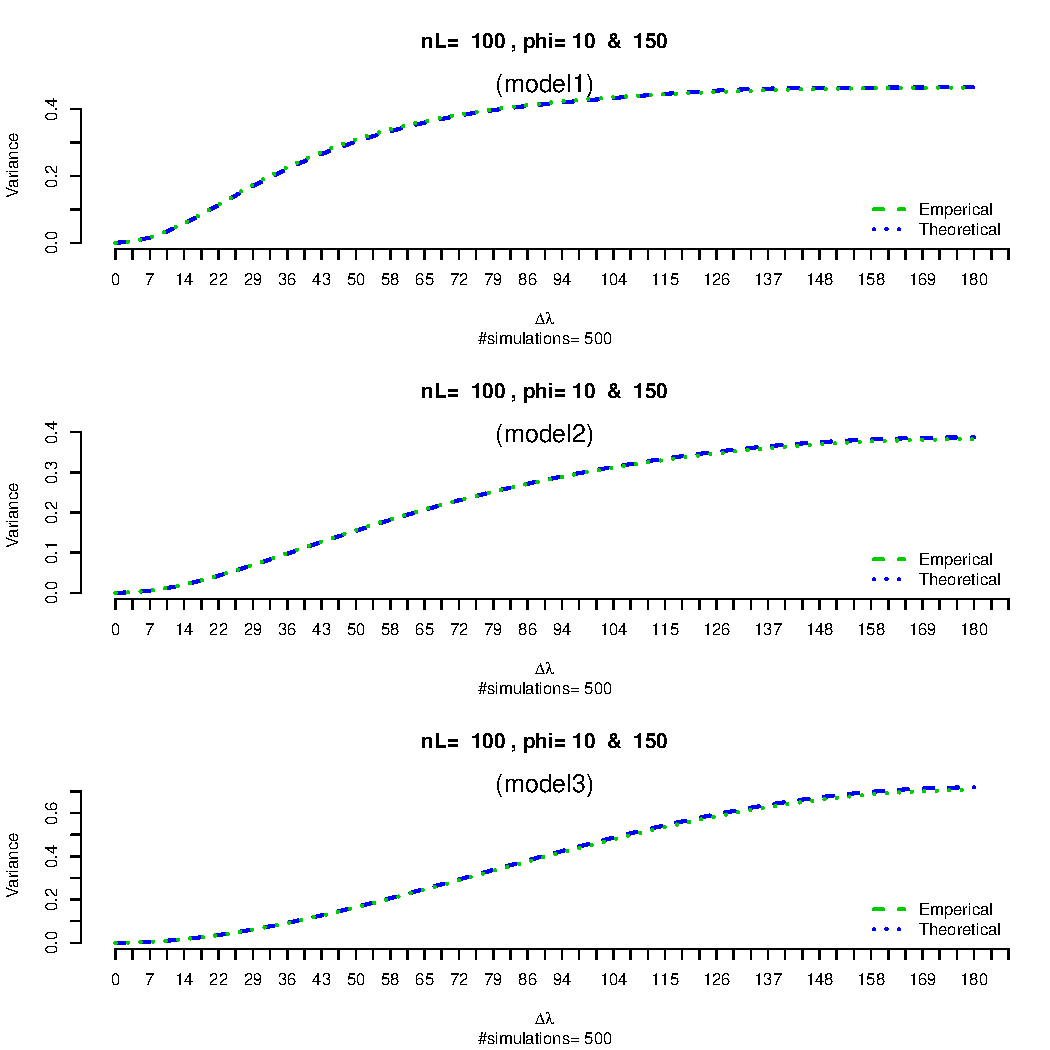
\includegraphics [width=0.9\textwidth ]{graphs/results_variogram_comparison}
	\includegraphics [scale =.9, keepaspectratio]{graphs/results_variogram_comparison_cm}
	% width=12cm,height=12cm
	\caption[Based on $C_m$ Approach the Cross Variogram Estimator Comparison]{Based on $C_m$ approach the cross variogram estimator comparison for longitudinally reversible process using  model 1, model 2, and model 3 (when $u=0$).}
	\label{logitudinal_comparison_cm}
\end{figure}


%-------------------------------------%
\subsection{Comparison of Cross Covariance}
%-------------------------------------%

As indicated from Chapter 4, when $C_0(\phi_P, \phi_Q) = 0$, the cross covariance MOM estimator is unbiased. Therefore we obtain the cross covariance MOM estimates given by \eqref{cross_covariance} under model 2 and model 3, and then compare them with the true values. Here we select two pairs of latitudes, $\phi = 70, 80$ ($20^0S$ ,$10^0S$) and $\phi = 60, 120$ ($30^0S$, $40^0N$). One can note that the cross covariance estimates match with the theoretical values very well (Figure \ref{cross_cov_comparison}).

%% individual cross covaraiance graphs
% \begin{figure}[H]
% \begin{center}
% 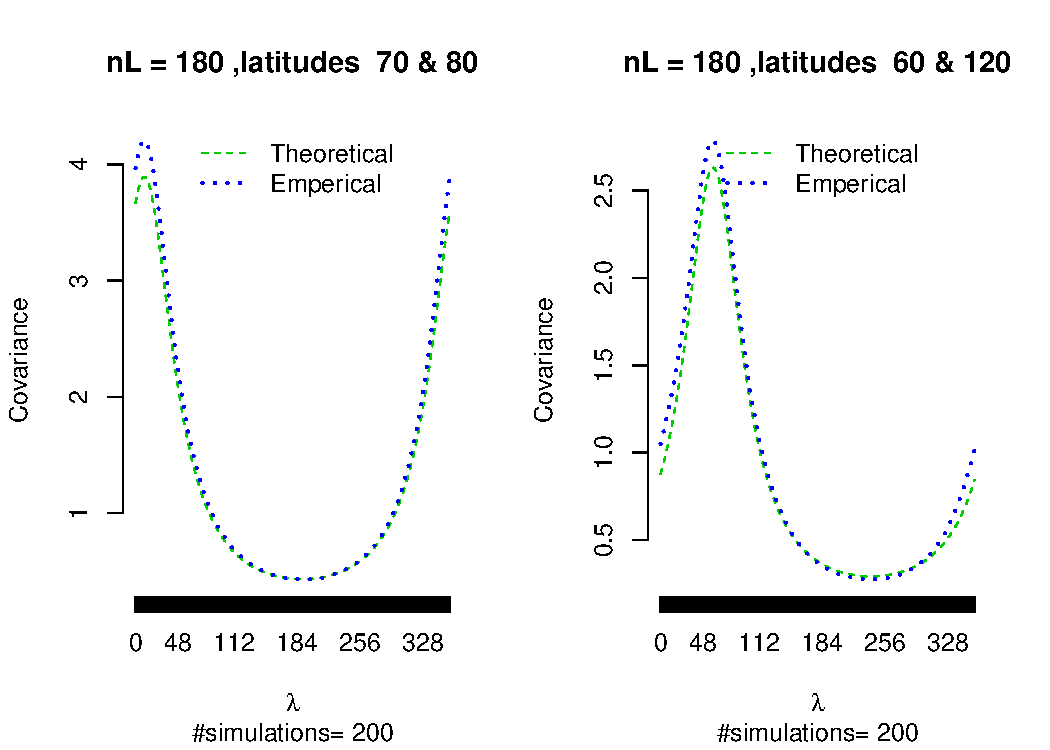
\includegraphics [width=0.75\textwidth ]{graphs/Model1.pdf}
% \caption{Cross covariance comparison of model1}
% \end{center}
% \end{figure}

% \begin{figure}[H]
% 	\begin{center}
% 		\includegraphics [width=0.75\textwidth ]{graphs/Model2.pdf}
% 		%\includegraphics [width=6in, height=3in]{Model2.pdf}
% 		\caption{Cross covariance comparison of model 2}
% 	\end{center}
% \end{figure}
% 
% 
% \begin{figure}[H]
% 	\begin{center}
% 		%\includegraphics [scale=.6]{Model3.pdf}
% 		\includegraphics [width=0.75\textwidth ]{graphs/Model3.pdf}
% 		\caption{Cross covariance comparison of model 3}
% 	\end{center}
% \end{figure}

\begin{figure}
	\begin{subfigure}{1\textwidth}
		\centering
		\includegraphics[keepaspectratio, scale=0.6]{graphs/Model2}
		\caption{Model 2 \eqref{model2}}
		\label{fig:cov2}
	\end{subfigure}
	\begin{subfigure}{1\textwidth}
		\centering
		\includegraphics[keepaspectratio, scale=0.6]{graphs/Model3}
		% \includegraphics[width=1\linewidth]{graphs/Model3}
		\caption{Model 3 \eqref{model3}}
		\label{fig:cov3}
	\end{subfigure}
\caption[Cross Covariance Comparison of Model 2 and Model 3]{Cross covariance comparison of model 2 and model 3}
\label{cross_cov_comparison}
\end{figure}


%-------------------------------------%
\subsection{Comparison of MSE}
%-------------------------------------%

In addition to comparing the biases, we also consider the mean square error (MSE) of the MOM cross variogram estimates obtained under both $C_m$ and direct $R(P,Q)$ approaches. The overall MSE is calculated based on the following formula.
\begin{eqnarray*}
MSE &=& \frac{1}{n_L} \sum (var + bias^2) \\
    &= & \frac{1}{n_L} \sum_{j=1}^{n_L} \left[ \frac{1}{nn}\sum_{i=1}^{nn}\left(\hat{\gamma_{i}}(j\delta)-\overline{\hat{\gamma}(j\delta)})^2\right) +  (\gamma_(j\delta) - \overline{\hat{\gamma}(j\delta)})^2 \right]
\end{eqnarray*}

\noi where $\delta = \frac{2\pi}{n_L}$ and $nn$ is the number of simulations.

\begin{figure}[H]
	\begin{subfigure}{.5\textwidth}
		\centering
		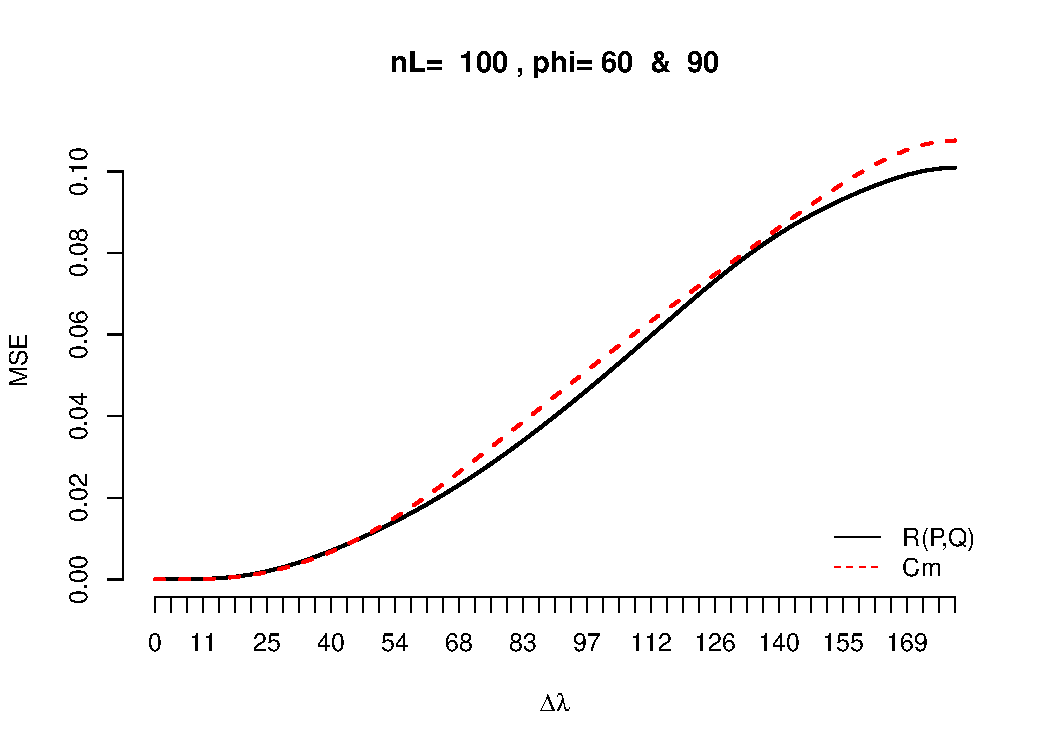
\includegraphics[width=1\linewidth]{graphs/MSE_comparison_model1_60_90}
		\caption{Model 1 (pair 1)}
		\label{fig:mse1}
	\end{subfigure}
	\begin{subfigure}{.5\textwidth}
		\centering
		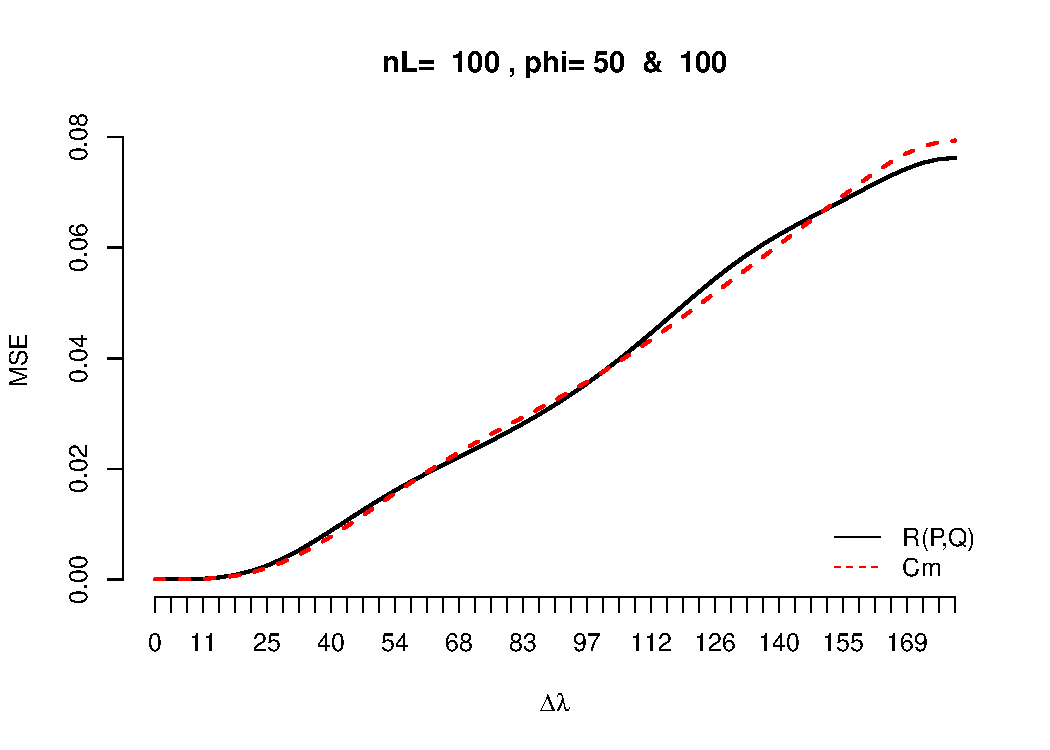
\includegraphics[width=1\linewidth]{graphs/MSE_comparison_model1_50_100}
		\caption{Model 1 (pair 2)}
		\label{fig:mse2}
	\end{subfigure}
		\begin{subfigure}{.5\textwidth}
		\centering
		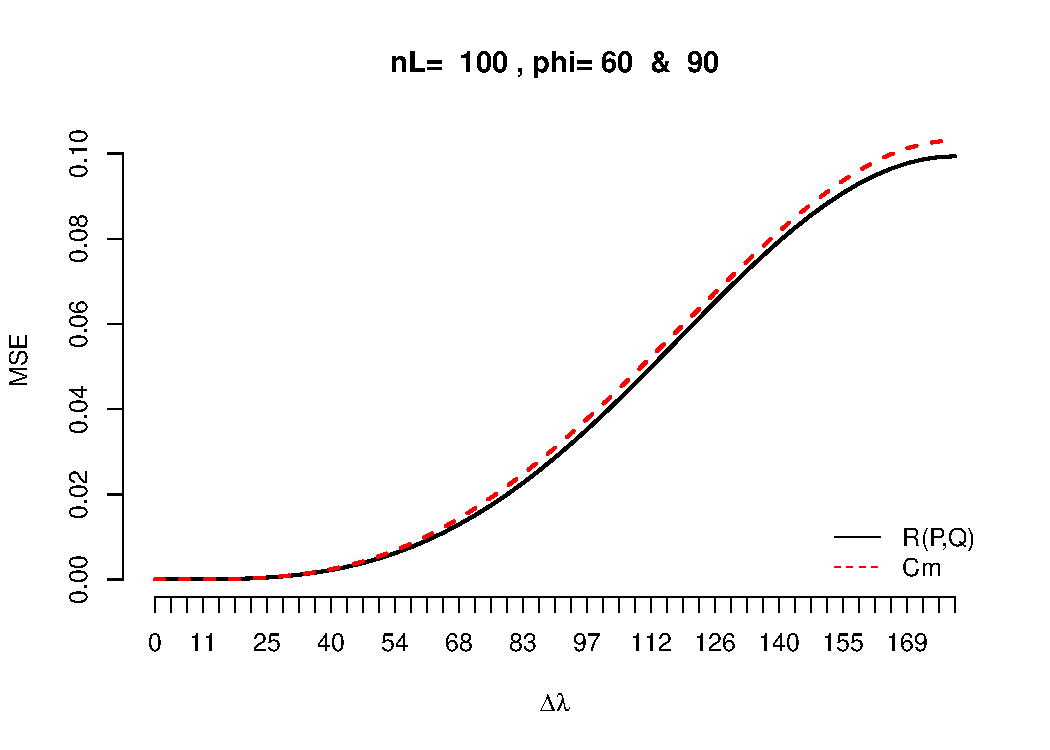
\includegraphics[width=1\linewidth]{graphs/MSE_comparison_model2_60_90}
		\caption{Model 2 (pair 1)}
		\label{fig:mse3}
	\end{subfigure}
		\begin{subfigure}{.5\textwidth}
		\centering
		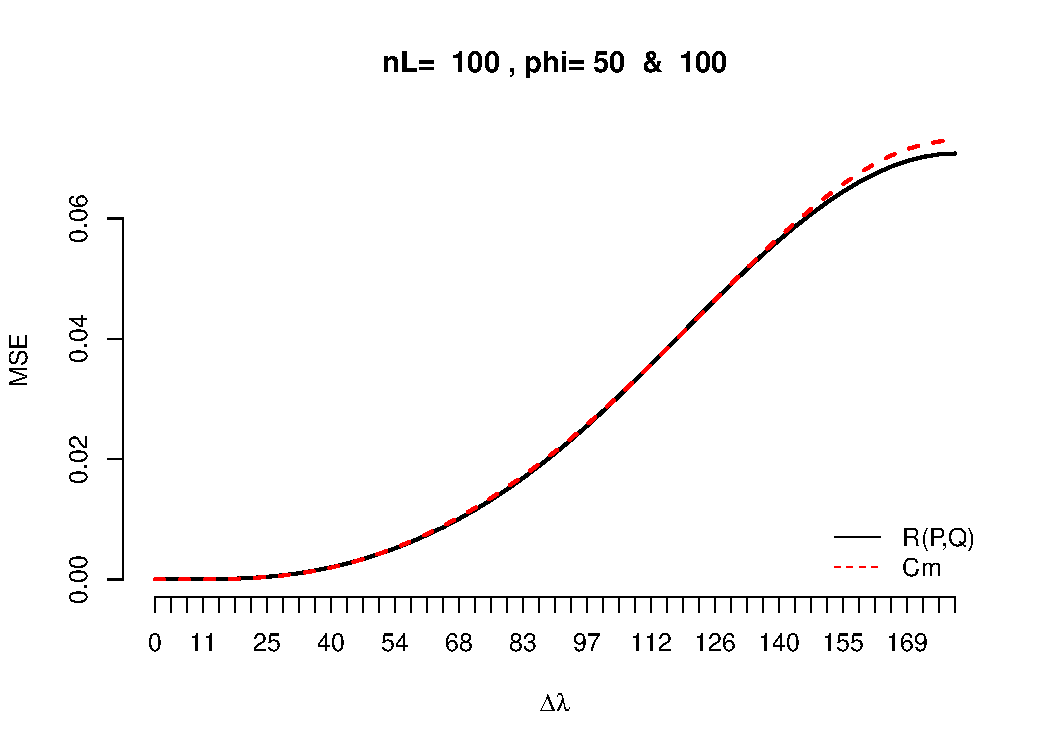
\includegraphics[width=1\linewidth]{graphs/MSE_comparison_model2_50_100}
		\caption{Model 2 (pair 2) }
		\label{fig:mes4}
	\end{subfigure}
	\caption[MSE Comparison Between $C_m$ and $R(P,Q)$ Using 500 Simulations]{MSE comparison between $C_m$ and $R(P,Q)$ using 500 simulations; pair 1 ($30^0S,0^0$), pair 2 ($40^0S, 10^0N$) figures (a) - (b) is the comparison for model 1 and figure (c)-(d) is the comparison for model 2 }
	\label{mse_comparison}
\end{figure}

\begin{table}[H]
\label{parameters}
\centering
\caption[MSE Comparison for $C_m$ and $R(P,Q)$ Approaches, the Values in Paranthesis]{MSE comparison for $C_m$ and $R(P,Q)$ approaches, the values in paranthesis are the bias for each pair.  Set 1 and Set 2 are referring to the set of parameters discussed in simulation setup}
\vskip 16pt
\begin{tabular}{|l|c|l|l|l|l|}
\hline
\multicolumn{2}{|c|}{}      & \multicolumn{2}{|c|}{Set 1} & \multicolumn{2}{|c|}{Set 2}  \\ \hline
Model & $(\phi_P, \phi_Q)$  & $R(P,Q)$  & $C_m$           & $R(P,Q)$  & $C_m$  \\ \hline
\multirow{6}{*}{Model1} & \multirow{2}{*}{(60, 90)}  & 2.298    & 2.427	  & 15.688	& 16.384	 \\
                        & &                            (0.0022) & (0.0004)& (0.0250)& (0.0015)	\\ \cline{2-6}
                        & \multirow{2}{*}{(50, 100)} & 1.784    & 1.782	  & 13.295 	& 12.767 	 \\
                        & &                            (0.0009) &(0.0001) & (0.0193)& (0.0030) 	 \\ \cline{2-6}
                        & \multirow{2}{*}{(10, 150)} & 0.564    & 0.623	  & 8.062	  & 9.177	 \\ 
                        & &                            (0.0009) &(0.0001) & (0.0226)& (0.0023)	 \\ \hline
\multirow{6}{*}{Model2} & \multirow{2}{*}{(60, 90)}  & 2.000    & 2.080	  & 12.452	& 13.021	 \\
                        & &                            (0.0004) & (0.0004)& (0.0042) & (0.0023)	\\ \cline{2-6}
                        & \multirow{2}{*}{(50, 100)} & 1.437    & 1.459	  & 9.196	  & 9.262 	 \\
                        & &                            (0.0001) &(0.0000) & (0.0015)& (0.0006) 	 \\ \cline{2-6}
                        & \multirow{2}{*}{(10, 150)} & 0.457    & 0.512	  & 6.034	  & 7.266	 \\ 
                        & &                            (0.0014) &(0.0001) & (0.0337)& (0.0026)	 \\ \hline
\end{tabular}
\end{table}

One can see from the above table that a variety of pairs of latitudes and two different sets of parameters are used in simulations. The MSEs from $C_m$ are comparable with those from direct $R(P,Q)$ approach while the $C_m$ approach gives smaller bias.



%
% \[
% MSE = \frac{1}{n_L-1}\sum_{k=1}^{n_L} (\gamma_{k}(\Delta\lambda) - \overline{\hat{\gamma}_{k}(\Delta\lambda)})^2
% \]

% \begin{table}[H]
% \label{parameters}
% \centering
% \begin{tabular}{|l|l|l|l|l|l|l|}
% \hline
%  & \multicolumn{2}{|c|}{Model 1} & \multicolumn{2}{|c|}{Model 2} & \multicolumn{2}{|c|}{Model 3} \\ \cline{2-7}
% Parameters & $R(P,Q)$  & $C_m$  & $R(P,Q)$  & $C_m$ & $R(P,Q)$  & $C_m$ \\ \hline
% % set 1 & 	0.04825 & 0.00881   & 	0.01820 & 0.00534 & 	-- & 0.01426 \\
% % set 2 & 	1.15598 & 0.16591   & 	0.42931 & 0.14270 & 	-- & 0.33726 \\ \hline \hline
%
% set 1 & 0.000965 &  0.0001762	& 0.000364	& 0.000107	&--&	0.0002852 \\
% set 2 & 0.023119 &  0.0033182	& 0.0085862	& 0.002854	&--&	0.0067452 \\ \hline \hline
%
% %model 1 4000 Cm 0.03085625
% %model 1 4000 R(P,Q) 0.1144611
%
% \end{tabular}
% \caption{MSE comparison}
% \end{table}

% Now the MSE for $R(P,Q)$ is lower but the bias is higer (bias for $C_m = 0.0325219$ and $R(P,Q) = 0.2493109$.)


%-------------------------------------%
\subsection{Generated Data}
%-------------------------------------%

\begin{figure}[H]
	\centering
		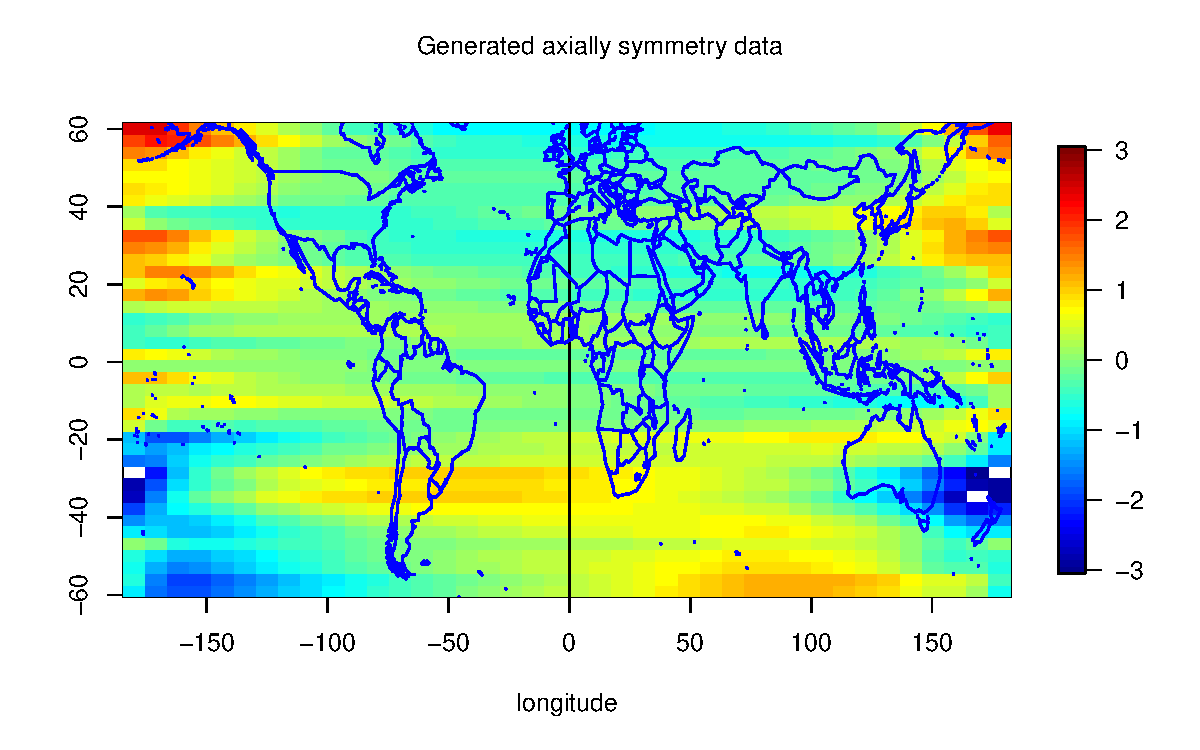
\includegraphics [width=1\textwidth ]{graphs/Data_sample_120_model2_withmap.pdf}
		\caption[A Snapshot of Global Data Generated Based on $C_m$ Approach using Zero]{A snapshot of global data generated based on $C_m$ approach using zero mean random process (model 2)}
		\label{grid_plot_model_2}
\end{figure}
The Figure \ref{grid_plot_model_2} is a snapshot of the global data generated based on model 2 and could potentially be used later for research. Clearly there are spatial trends within the latitudes but not within longitudes. It is somewhat difficult to use the covariance structure to generate data when it is closer to Earth's pole (similar complexity can also be observed in MSU and TOMS data). Therefore we produced a snapshot by generating the data on $[0,2\pi/3] \times [0,2\pi]$ (equivalent to $[-\pi/3,\pi/3] \times [-\pi,\pi]$ ) grid, with a grid resolution of $1^0\times 2^0$ ({\em i.e } $n_l = 120, n_L=180 \Rightarrow$ 21600 spatial points). However we observed some inconsistencies (strong spots) when examining closer close to the boundary points of longitudes ($\lambda \rightarrow \pm \pi$).

\begin{figure}[H]
	\begin{center}
		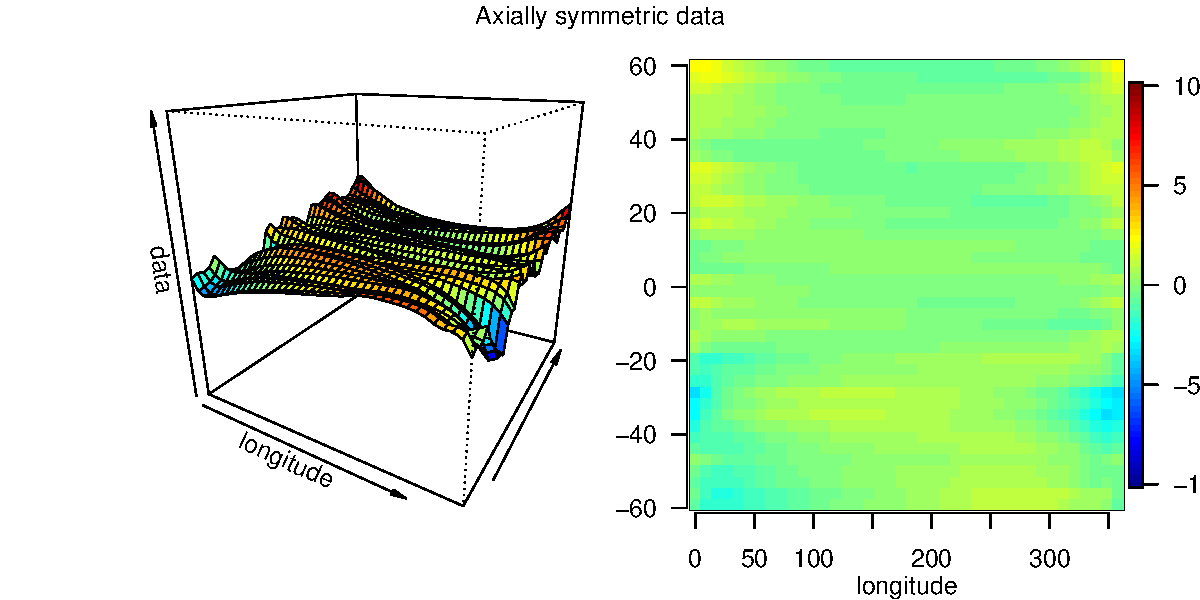
\includegraphics [width=0.9\textwidth ]{graphs/Data_sample_120_model2_density.pdf}
		\caption[One Snapshot of The Axially Symmetric Data Generated Based on Model 2]{One snapshot of the axially symmetric data generated based on model 2, grid resolution $2^0\times 1^0$ (data scale -10 and 10).}
			\label{grid_plot_model2_sim2}
	\end{center}
\end{figure}
The above Figure \ref{grid_plot_model2_sim2} refers to the data snapshot given by Figure \eqref{grid_plot_model_2} and it is clear that trends are within latitudes not within longitudes. Four snapshots of the gridded data generated based on all models are given in Appendix \ref{appendixA}.

%\end{document}
